\chapter{\LaTeX{}模板及论文撰写说明}\label{cha:3}

\section{模板基本结构与调整说明}

\subsection{模板目录与结构清单}
模板目录与结构清单如\tabref{模板目录与结构清单}所示。


\begin{table}[H]\wuhao
  \centering
  \renewcommand\arraystretch{0.8} % 行距
  \bitabcaption{模板目录与结构清单}{List of Template Catalogs and Structures}
  \begin{tabular}{ll}
    \toprule
    文件名          & 描述                         \\
    \midrule
    chapters & 论文章节存放目录  \\
    figures & 论文插图存放目录        \\
    bjtumaster.cls   & 模板文件                     \\
    main.tex & 论文主文档    \\
    betterbib.bib & 论文参考文献库(BibLaTeX)        \\
    gbt7714-numerical.bst & BibTeX 参考文献表国标样式文件    \\
    bibspacing.sty & 参考文献间距调整宏包  \\
    \bottomrule
  \end{tabular}
  \label{模板目录与结构清单}
\end{table}

使用本模板时,请在\cs{chapters}目录下删改、新增并编辑论文的章节\cs{*.tex}文件;在\cs{figures}目录下上传论文的插图;在\cs{main.tex}文件内编辑论文的整体结构;在\cs{betterbib.bib}内编辑论文引用文献的条目信息。若有需求可修改\cs{bjtumaster.cls}文件内的论文的版面结构设置。

\subsection{封面页、学位论文版权使用授权书}
需要编辑\cs{chapters}\cs{cover.tex}文件。封面页为第一部分,需\textbf{论文中、英文标题,作者,导师}四个字段。日期会自动生成,毋需编辑。学位论文版权使用授权书为第二部分,可编辑日期。签名建议脱离\LaTeX{}环境后插入或手写。

\subsection{题名页}
需要编辑\cs{chapters}\cs{cover2.tex}文件内\textbf{密级、论文中、英文标题,作者姓名、学号,导师姓名、职称,学位类别、级别,学科专业,研究方向}十一个字段。日期会自动生成,毋需编辑。

\subsection{致谢}
请在\cs{chapters}\cs{ack.tex}文件内编写。

\subsection{中英文摘要、序言}
请在\cs{chapters}\cs{abstract.tex}文件内编写。若无需序言请删除以下字段:

\begin{lstlisting}[language={[LaTeX]TeX}]
    \chapter*{序言(若有)}
    \markboth{序言}{}
    ......
\end{lstlisting}

\subsection{目录、插图清单、附表清单}
毋需手动编辑,若无插图清单、附表清单使用需求,请在\cs{main.tex}文件内删除以下字段:
\begin{lstlisting}[language={[LaTeX]TeX}]
    \cleardoublepage            % 若有图清单
    \listoffigures              % 若有图清单
    {(可根据需要撰写或移除)如学位论文中图表较多,应分别列出清单置于目录页之后。图的清单应有序
    号、图题和页码;表的清单应有序号、表题和页码。 } % 需要删除
    
    \cleardoublepage            % 若有附表清单
    \listoftables               % 若有附表清单
    {(可根据需要撰写或移除)如学位论文中图表较多,应分别列出清单置于目录页之后。图的清单应有序
    号、图题和页码;表的清单应有序号、表题和页码。 } % 需要删除
\end{lstlisting}

\subsection{术语表}
本模板提供了术语表功能,用于整理论文中的物理常数、概念与缩写、数学符号等内容。请在\cs{chapters}\cs{nomenclature.tex}文件内编辑。基本语法有三种,分别为:

\begin{lstlisting}[language={[LaTeX]TeX}]
    \nomenclature[类别]{术语}{描述}
    \nomenclature[类别, 强制排序编号]{术语}{描述}
    \nomenclature[类别, 强制排序编号]{术语}{描述}\nomunit{\SI[group-digits=false]{数值}{单位}}
\end{lstlisting}

类别包含:A:物理常数;B:概念与缩写;C:数学符号。强制排序编号为数值,如\texttt{01},可留空。对特殊物理常数可添加其常数数值与单位。

若有需求,可进入\cs{bjtumaster.cls}文件内编辑术语类别,具体定义语句为:
\begin{lstlisting}[language={[LaTeX]TeX}]
    \renewcommand\nomgroup[1]{%
        \item[\hei
        \ifstrequal{#1}{A}{物理常数}{%
        \ifstrequal{#1}{B}{概念与缩写}{%
        \ifstrequal{#1}{C}{数学符号}{}}}%
        ]\vspace{1em} % 在类别标题之后增加 1em 间距
    }
\end{lstlisting}

若无术语表使用需求,请在\cs{main.tex}文件内删除以下字段:

\begin{lstlisting}[language={[LaTeX]TeX}]
    \cleardoublepage            % 若有术语表
    \nomenclature[A, 01]{$g_\mathrm{pk}{}$}{{北京地区重力加速度}
    \nomunit{\SI[group-digits=false]{9.80151}{\mathrm{kg}/\mathrm{s}^2}}}


    
\nomenclature[B,01]{BJTU}{北京交通大学}
\nomenclature[B,02]{MECE}{机械与电子控制工程学院}
\nomenclature[B,03]{RRC}{机器人研究中心}
\nomenclature[B,04]{\TeX{}}{一个优秀的排版工具,擅长于对于复杂数学符号的处理}
\nomenclature[B,05]{\LaTeX{}}{一种基于\TeX{}的排版系统}
\nomenclature[B,06]{\XeTeX{}}{一种使用Unicode的\TeX{}排版引擎,并支持一些现代字体技术}
\nomenclature[B,07]{\overleaf{}}{一个云端协作式\LaTeX{}编辑器,可用于编写和发布论文。}



\nomenclature[C]{$M$}{机构自由度}
\nomenclature[C]{$d$}{机构维数}
\nomenclature[C]{$g$}{运动副数目}
\nomenclature[C]{$f_k$}{第$k$运动副的自由度数}
\nomenclature[C]{$\xi$}{局部自由度}
   % 若有术语表
    \printnomenclature          % 若有术语表
\end{lstlisting}

\subsection{主体部分}
请直接在\cs{chapters}目录内编辑、新建\cs{chapters0x.tex},正常标题创建方式为:
\begin{lstlisting}[language={[LaTeX]TeX}]
\chapter{章(一级)标题}
\section{节(二级)标题}
\subsection{三级标题}
\subsubsection{四级标题(编号)}
\end{lstlisting}

若有引用需求请在各级标题后立即创建标签便于后续引用,标签名自行定义,语句为:
\begin{lstlisting}[language={[LaTeX]TeX}]
\lable{标签名}
\end{lstlisting}


在\cs{main.tex}文件中在合适位置使用语句调用\cs{chapters}\cs{chapters0x.tex}文件并进行编译,其语句为:
\begin{lstlisting}[language={[LaTeX]TeX}]
\input{chapters/chapter0x}
\end{lstlisting}

正文中的标号按如下编号格式顺序排列:先(1)、(2)、(3), 再1)、2)、3),后\numcircled{1}、\numcircled{2}、\numcircled{3},标号后避免出现标点符号、英文字母、 PPT中的项目符号。

带圈数字仅支持1$\sim$10的数字输入,输入语句为:
\begin{lstlisting}[language={[LaTeX]TeX}]
\numcircled{数字}
\end{lstlisting}

可使用\cs{mypara{}}命令插入含加粗小标题的段落,例如:

\mypara{海猫络合物} 中国插画家、同人创作者及游戏《明日方舟》制作人,业余平面设计师与建筑师。现居上海市。毕业于浙江杭州高级中学、中国美术学院建筑系,前少女前线首席游戏图形设计师(主美),鹰角网络创始人之一。

可使用\cs{itemize}环境创建不编号列表,例如:

\begin{itemize}
    \item \textbf{智力:}逻辑思维、博学多闻、能说会道、故弄玄虚、标新立异、见微知著
    \item \textbf{精神:}平心定气、内陆帝国、通情达理、争强好胜、同舟共济、循循善诱
    \item \textbf{体格:}钢筋铁骨、坚忍不拔、强身健体、食髓知味、天人感应、疑神疑鬼
    \item \textbf{身手:}眼明手巧、五感发达、反应速度、鬼祟玲珑、能工巧匠、从容自若
\end{itemize}

可使用\cs{enumerate}环境创建编号列表,例如:

\begin{enumerate}
    \item \textbf{警探巨星:}说超级巨星台词7次
    \item \textbf{新自由主义街区天字第一号皮条客:}吹捧自由市场9次
    \item \textbf{招募曷城金警探:}57区的杰出代表
    \item \textbf{世界上最可怜的警探:}道歉10次
    \item \textbf{雕像也无法让她回心转意:}它们毫无意义
    \item \textbf{传统主义疯狗:}说传统主义事项10次
    \item \textbf{无聊之极:}说极其无聊之事7次
    \item \textbf{法律化身:}说你就是法律7次
\end{enumerate}

可使用\texttt{[label=(\textbackslash arabic*)]}、\texttt{[label={[}\textbackslash Roman*{]}]}等指令修改enumerate编号列表的编号格式,如:

\begin{enumerate}[label=(\arabic*)]
    \item \textbf{费尔韦瑟T-500搪瓷套装:}从头到脚,全副武装
    \item \textbf{第八封印的开启者:}警告他人末日即将来临8次
    \item \textbf{现界之敌:}教训5件静物
    \item \textbf{招募警探库诺·德鲁伊特:}下级警官的料
    \item \textbf{超级遥视者:}得见幕外6次
    \item \textbf{机械痴:}闲扯关于机械的话题4次
\end{enumerate}

\begin{enumerate}[label={[}\Roman*{]}]
    \item \textbf{模范坏警察:}与金一起创下历史新低
    \item \textbf{挑战硬核:}祝你好运
    \item \textbf{大陆荣誉警察:}获得11点荣耀点数
    \item \textbf{无谷蛋白顶料馅饼:}接下来你就要切断碳水化合物了
    \item \textbf{真探:}以硬核模式通关游戏
    \item \textbf{灰域行者:}切换次元3秒钟
\end{enumerate}

\subsection{作者简历及攻读学位期间取得的研究成果}
需要编辑\cs{chapters}\cs{Curriculum Vitae.tex}文件。

书写格式与参考文献相同,页码后需注明该文章对应学位论文的章节序号。
如已发表的学术论文被EI或SCI收录,请标明收录号;SCI论文一般应标注发表
当年的影响因子;对已录用但尚未发表的学术论文,请注明是否EI或SCI刊源。

\subsection{独创性声明、学位论文数据集}
独创性声明签名建议脱离\LaTeX{}环境后插入或手写。学位论文数据集需要编辑\cs{chapters}\cs{statement.tex}文件内表格信息。

\section{论文中的图、表、引用等多元内容的使用}

\subsection{插图}
图片通常在figure环境中进行插入。建议矢量图片使用PDF或SVG格式,比如数据可视化的绘图;建议非矢量图片使用PNG或JPG格式插入。注意,\LaTeX{}不支持TIFF格式;EPS格式已经过时。

图应有“自明性”。插图应与文字紧密配合,文图相符,内容正确。选图要力求精练,插图、照片应完整清晰。

照片图要求主题和主要显示部分的轮廓鲜明,如\figref{fig:eg1}所示,便于制版。如用放大或缩小的
复制品,必须清晰,反差适中。照片上应有表示目的物尺寸的标度。

\begin{figure}[htbp]
  \centering
  
\includegraphics[width=0.5\linewidth]{example-image-a.pdf}
  \bifigcaption{图片示例\cite{TUN2025LaTeXThesisTe}}{Example Image\cite{TUN2025LaTeXThesisTe}}
  \label{fig:eg1}
\end{figure}

引用文献中的图\cite{TUN2025LaTeXThesisTe}时,除在正文文字中标注参考文献序号以外,还必须在中、
英文图题的右上角标注参考文献序号。

图中若有子图时,如\figref{fig:eg2}所示,子图题置于子图之下或图题之下,用中、英文书写,子图
号用a)、b)等表示。

\begin{figure}
  \centering
  \subcaptionbox{子图 A\protect\\ \thesubfigure\, Subfigure A\label{fig:subfig-a}}
    {
\includegraphics[width=0.35\linewidth]{example-image-a.pdf}}
  \subcaptionbox{子图 B\protect\\ \thesubfigure\, Subfigure B\label{fig:subfig-b}}
    {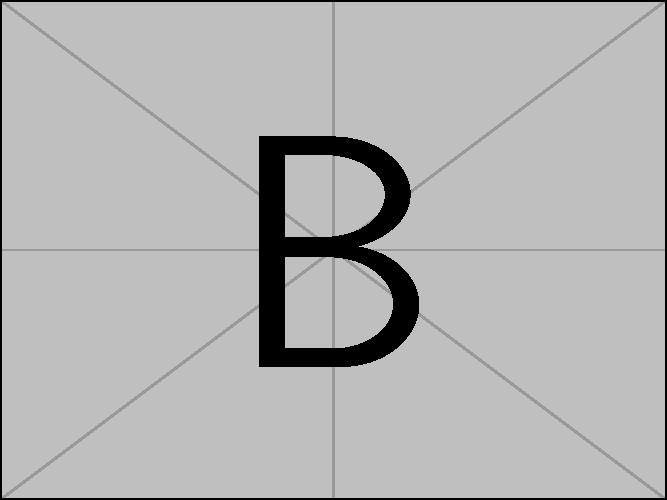
\includegraphics[width=0.35\linewidth]{example-image-b.pdf}}
  \bifigcaption{多个子图的示例}{Example of Multiple Subfigures}
  \label{fig:eg2}
\end{figure}

图中各部分说明应采用中文(引用的外文图除外)或数字符号,各项文字说明
置于图题之上(有子图时,置于子图题之上)。

图中文字用宋体(中文)或Times New Roman 字体(西文),字号尽量采用五号字(当字数较多时可用小五,以清晰表达为原则,但在一个插图内字号要统一)。同一图内使用文字应统一。

插图之前,文中必须有关于本插图的提示,如“见图1-1”、“如图1-1所示”
等。插图与其图题为一个整体,不得拆开排写于两页。插图处的该页空白不够排
写该图整体时,则可将其后文字部分提前排写,将图移到次页。有子图时,子图
过多在一页内安排不下时,可转到下页,总图题只出现在下页。

为了实现北京交通大学论文格式要求的双语图名,必须使用本文规定格式进行图片插入。以\figref{fig:eg1},\figref{fig:eg2}为例,对于*.pdf、*.jpg、*.png等格式图片插入代码格式为:

\begin{lstlisting}[language={[LaTeX]TeX}]
\begin{figure}[位置控制]
  \centering
  
\includegraphics[显示宽度]{example-image-a.pdf(文件名)}
  \bifigcaption{中文图名}{英文图名}
  \label{标签名}
\end{figure}

\begin{figure}[位置控制]
  \centering
  \subcaptionbox{{子图中文图名1}\protect\\ \thesubfigure\, {子图英文图名1}\label{子图标签名1}}
    {\includegraphics[显示宽度]{文件名1}}
  \subcaptionbox{{子图中文图名2}\protect\\ \thesubfigure\, {子图英文图名2}\label{子图标签名2}}
    {\includegraphics[显示宽度]{文件名2}}
  \bifigcaption{总图中文名}{总图英文名}
  \label{总图标签名}
\end{figure}
\end{lstlisting}

\noindent 其中“[]”内可设置的属性字段请查阅\LaTeX{}的graphics宏包文档\cite{CP2024Packagesgraphi},此处不再赘述。

若插入*.svg格式的矢量图,则不可使用\cs{includegraphics}命令,如矢量\figref{猪肉刺身杯},其插入代码应修改为:

\begin{figure}[H]
  \centering
  \includesvg[width=7cm]{example-svg.svg}
  \bifigcaption{svg插入示例(Zeto设计)}{Example of svg (designed by Z.T. YEUNG)}
  \label{猪肉刺身杯}
\end{figure}

\begin{lstlisting}[language={[LaTeX]TeX}]
\begin{figure}[位置控制]
  \centering
  \includesvg[显示宽度]{svg文件名}
  \bifigcaption{中文图名}{英文图名}
  \label{标签名}
\end{figure}
\end{lstlisting}

\subsection{插表}
表应有“自明性”。表应有表题,表题即表的名称,置于表的编号之后。

表格不加左、右边线。表的编排建议采用国际通行的三线表,如\tabref{tab:eg1}。表中文字用宋
体(中文)或Times New Roman字体(英文),字号尽量采用5号字(当字数较多
时可用小5号字,但在一个插表内字号要统一)。 

表头设计应简单明了,尽量不用斜线。表头中可采用化学符号或物理量符号。 
全表如用同一单位,则将单位符号移至表头右上角,加圆括号。

表中数字空缺的格内加横线“—”(占2个半角字符)。表内文字或数字上、
下或左、右相同时,不允许用“〃”、“同上”之类的写法。 

表内文字说明,起行空2个半角字符,转行顶格,句末不加标点。

\begin{table}[H]\wuhao
  \centering
  \renewcommand\arraystretch{1.0} % 行距
  \bitabcaption{三线表示例\cite{TUN2025LaTeXThesisTe}}{Example Table\cite{TUN2025LaTeXThesisTe}}
  \begin{tabular}{ll}
    \toprule
    文件名          & 描述                         \\
    \midrule
    bjtumaster.cls   & 模板文件                     \\
    main.tex & 论文主文档    \\
    chapters & 论文章节存放目录  \\
    figures & 论文插图存放目录        \\
    betterbib.bib & 论文参考文献库(BibLaTeX)        \\
    gbt7714-numerical.bst & BibTeX 参考文献表国标样式文件    \\
    bibspacing.sty & 参考文献间距调整宏包  \\
    \bottomrule
  \end{tabular}
  \label{tab:eg1}
\end{table}

插表之前文中必须有相关文字提示,如“见表1-1”、“如表1-1所示”。一般
情况下插表不能拆开两页编排,如某表在一页内安排不下时,才可转页,以续表
形式接排。表右上角注明编号,编号后加“(续表)”,并重复表头,如\tabref{tab:eg2}所示。
插表的上下与文中文字间需空一行编排。 

引用文献中的表格时,除在正文\cite{TUN2025LaTeXThesisTe}文字中标注参考文献序号以外,还必须在中、
英文表题的右上角标注参考文献序号。

% 在 longtable 之前定义表清单标题(隐藏)
\begin{table}[H]
  \bitabcaption{跨页长表格}{Long Tables Across Pages}
  \label{tab:eg2}
\end{table}
\vspace{-1cm}
\addtocounter{table}{-1} % 回退表格计数器
\begin{longtable}{cccc}
    \toprule
    表头 1 & 表头 10 & 表头 11 & 表头 100 \\
    \midrule
  \endfirsthead
    \caption*{续表~\thetable\quad {跨页长表格}\vspace{-0.8cm}} \\
    \caption*{Continued Table~\thetable\quad {Long Tables Across Pages}} \\
    \toprule
    表头 1 & 表头 10 & 表头 11 & 表头 100 \\
    \midrule
  \endhead
    \bottomrule
  \endfoot
  Row 1  & & & \\
  Row 2  & & & \\
  Row 3  & & & \\
  Row 4  & & & \\
  Row 5  & & & \\
  Row 6  & & & \\
  Row 7  & & & \\
  Row 8  & & & \\
  Row 9  & & & \\
  Row A & & & \\
  Row B  & & & \\
  Row C  & & & \\
  Row D  & & & \\
  Row E & & & \\
  Row F & & & \\
  Row 10 & & & \\
  Row 11  & & & \\
  % Row 12  & & & \\
  % Row 13  & & & \\
  % Row 14 & & & \\
  % Row 15 & & & \\
  % Row 16 & & & \\
  % Row 17  & & & \\
  % Row 18  & & & \\
  % Row 19  & & & \\
  % Row 1A & & & \\
  % Row 1B & & & \\
  % Row 1C & & & \\
  % Row 1D  & & & \\
  % Row 1E  & & & \\
  % Row 1F  & & & \\
  % Row 20 & & & \\
\end{longtable}

本文非常不建议手搓表格代码,建议使用第三方插件如Create LaTeX tables online\cite{TabCreateLaTeXta}制作表格再拷贝进\LaTeX{}进行进一步处理,故不介绍普通表格插入命令。

若非不可抗力,尽量避免跨页长表格。对于跨页长表格,本模板为了实现中英文双语表题且在图清单内正常显示,采用了非常拙劣的办法。建议查看代码理解,具体步骤为:
\begin{enumerate}
    \item 使用\cs{begin\{table\}......}\cs{end\{table\}}定义一个双语表题(及标签)
    \item 使用\cs{vspace\{-1cm\}}减少表题与表格的间距
    \item 使用\cs{addtocounter\{table\}{-1}}回退表格计数器
    \item 使用\cs{begin\{longtable\}......}\cs{end\{longtable\}}定义跨页长表格。
\end{enumerate}
在第4)步中,需要再次输入一遍双语表题,具体修改部分为:

\begin{lstlisting}[language={[LaTeX]TeX}]
    \caption*{续表~\thetable\quad {中文表题}\vspace{-0.8cm}} \\
    \caption*{Continued Table~\thetable\quad {英文表题}} \\
\end{lstlisting}

在单元格内若需要进行换行操作,则需要使用\cs{makecell}宏包的指令,添加在需要换行的单元格上,如:

\begin{lstlisting}[language={[LaTeX]TeX}]
    \makecell{换行前的内容 \\ 换行后的内容}
\end{lstlisting}

\subsection{缩写、公式}

\subsubsection{缩写}
采用英语缩写词时,除本行业广泛应用的通用缩写词外,文中第一次出现的缩写词应该用括号注明英文原词。

\textbf{eg:} 自由度(Degree of Freedom, DoF)

\subsubsection{公式}
公式分为行内公式与行间公式两种。行内公式常用来表示简单物理量符号,不编号,有两种表示方法(后者不推荐),如“我们常用$\xi$表示机构局部自由度”的代码为:
\begin{lstlisting}[language={[LaTeX]TeX}]
我们常用$\xi$表示机构局部自由度
我们常用\(\xi\)表示机构局部自由度
\end{lstlisting}

行间公式可以使用\cs{equation}和\cs{equation*}环境,前者自动进行公式编号,后者不进行编号。若需要引用,则需要在公式开始后立即设置标签。
\vspace{2em}

\textbf{eg:}机构通用自由度公式\cite{HuangZhen2011LunJiGouZiYouDu}为:

\begin{equation}\label{自由度}
    M=d\left( n-g-1 \right) +\sum_{k=1}^g{f_k}+v-\xi
\end{equation}
式中,$d$为机构维数,$n$为构件数目,$g$为运动副数目,$\sum_{k=1}^g{f_k}$为各运动副自由度之和,$\xi$为局部自由度。

\equref{自由度}代码为:

\begin{lstlisting}[language={[LaTeX]TeX}]
\begin{equation}\label{自由度}
    M=d\left( n-g-1 \right) +\sum_{k=1}^g{f_k}+v-\xi =6\left( 5-4-1 \right) +4=4
\end{equation}
\end{lstlisting}

不编号行间公式亦可使用更快捷的\cs{[...}\cs{]或\$\$...\$\$}(后者不推荐)。

\textbf{eg:}空间任何一个矢量$\boldsymbol{s}$都可以由一个旋量$\textsl{\$}$来表达其方向和所在的空间位置\cite{GuoFang2007BingLianJiQiRenJiGouZongHeFangFaBiJiaoYanJiu},记作

\begin{equation*}
    \textsl{\$}=\left[  \begin{array}{c}
	               \boldsymbol{s}\\
	               \boldsymbol{s}_0+h\boldsymbol{s}\\
                    \end{array} \right] 
\end{equation*}

上式代码为:(论文中禁止使用“上式”、“上图”这种说法)
\begin{lstlisting}[language={[LaTeX]TeX}]
\begin{equation*}
    \textsl{\$}=\left[  \begin{array}{c}
	               \boldsymbol{s}\\
	               \boldsymbol{s}_0+h\boldsymbol{s}\\
                    \end{array} \right] 
\end{equation*}
或
\[
\textsl{\$}=\left[  \begin{array}{c}
	               \boldsymbol{s}\\
	               \boldsymbol{s}_0+h\boldsymbol{s}\\
                    \end{array} \right] 
\]
或
$$
\textsl{\$}=\left[  \begin{array}{c}
	               \boldsymbol{s}\\
	               \boldsymbol{s}_0+h\boldsymbol{s}\\
                    \end{array} \right] 
$$
\end{lstlisting}





较长的公式或多行公式需要转行时,应尽可能在“$=$”处回行,如\figref{自由度2},或者在“$+$”、“$-$”、“$\times$”、“$/$”等记号处对齐。

\begin{equation}\label{自由度2}
\begin{aligned}
    M &= d\left( n-g-1 \right) +\sum_{k=1}^g{f_k}+v-\xi \\
     &= 6\left( 5-4-1 \right) +4\\
     &= 4
\end{aligned}
\end{equation}

\equref{自由度2}代码为:

\begin{lstlisting}[language={[LaTeX]TeX}]
\begin{equation}\label{自由度2}
\begin{aligned}
    M &= d\left( n-g-1 \right) +\sum_{k=1}^g{f_k}+v-\xi \\
     &= 6\left( 5-4-1 \right) +4 \\
     &= 4
\end{aligned}
\end{equation}
\end{lstlisting}

公式中第一次出现的物理量代号应给予注释,注释的转行应与破折号“——”后第一个字对齐。破折号占4个半角字符,注释物理量需用公式表示时,公式后不应出现公式编号。

\subsection{算法、代码}

\subsubsection{算法}

算法环境使用\cs{algorithm}宏包,如\algref{alg1}的代码所示。

\begin{algorithm}
  \caption{Calculate $y = x^n$}
  \label{alg1}
  \small
  \begin{algorithmic}
    \REQUIRE $n \geq 0$
    \ENSURE $y = x^n$

    \STATE $y \leftarrow 1$
    \STATE $X \leftarrow x$
    \STATE $N \leftarrow n$

    \WHILE{$N \neq 0$}
      \IF{$N$ is even}
        \STATE $X \leftarrow X \times X$
        \STATE $N \leftarrow N / 2$
      \ELSE[$N$ is odd]
        \STATE $y \leftarrow y \times X$
        \STATE $N \leftarrow N - 1$
      \ENDIF
    \ENDWHILE
  \end{algorithmic}
\end{algorithm}

\subsubsection{代码}

代码提供行间代码与行内代码两种。行内代码适用场景较少,\\
如显示行内代码“\cs{input\{chapter03.tex\}}”的指令为:

\begin{lstlisting}[language={[LaTeX]TeX}]
\cs{input\{chapter03.tex\}}
\end{lstlisting}
\vspace{2em}
这是一段python代码,它作为行间代码显示在正文中:

\begin{lstlisting}[language={Python}]
def hello():
    print("Hello, World!")

hello()
\end{lstlisting}

显示这段python代码的指令为:

\begin{lstlisting}[language={[LaTeX]TeX}]
\begin{lstlisting}[language={Python}]
    def hello():
        print("Hello, World!")
    
    hello()
\end{lstlisting }
\end{lstlisting}

\subsection{引用}

\subsubsection{文献及电子资料}

论文中以任何形式引用的资料,均须标出引用出处,并以参考文献形式统一编号。引文标注遵照GB/T 7714-2005《文后参考文献著录规则\cite{QuanGuoXin2005WenHouCanKaoWenXianZhuLuGuiZe}》,采用顺序编码制。

当提及的参考文献为文中直接说明时,则用小4号字与正文排齐,如“由文献[2,4-7]可知”。

不得将引用文献标示置于各级标题处。

本文推荐采用BibLaTeX进行参考文献处理,即:对参考文献条目生成BibLaTeX格式的*.bib文件,将其内容拷贝至\cs{betterbib.bib}文件内。如文献管理软件Zotero可在安装betterbib插件后,在题录列表右键菜单内通过导出条目获得*.bib文件,如\figref{fig:zotero}所示。

\begin{figure}[htbp]
  \centering
  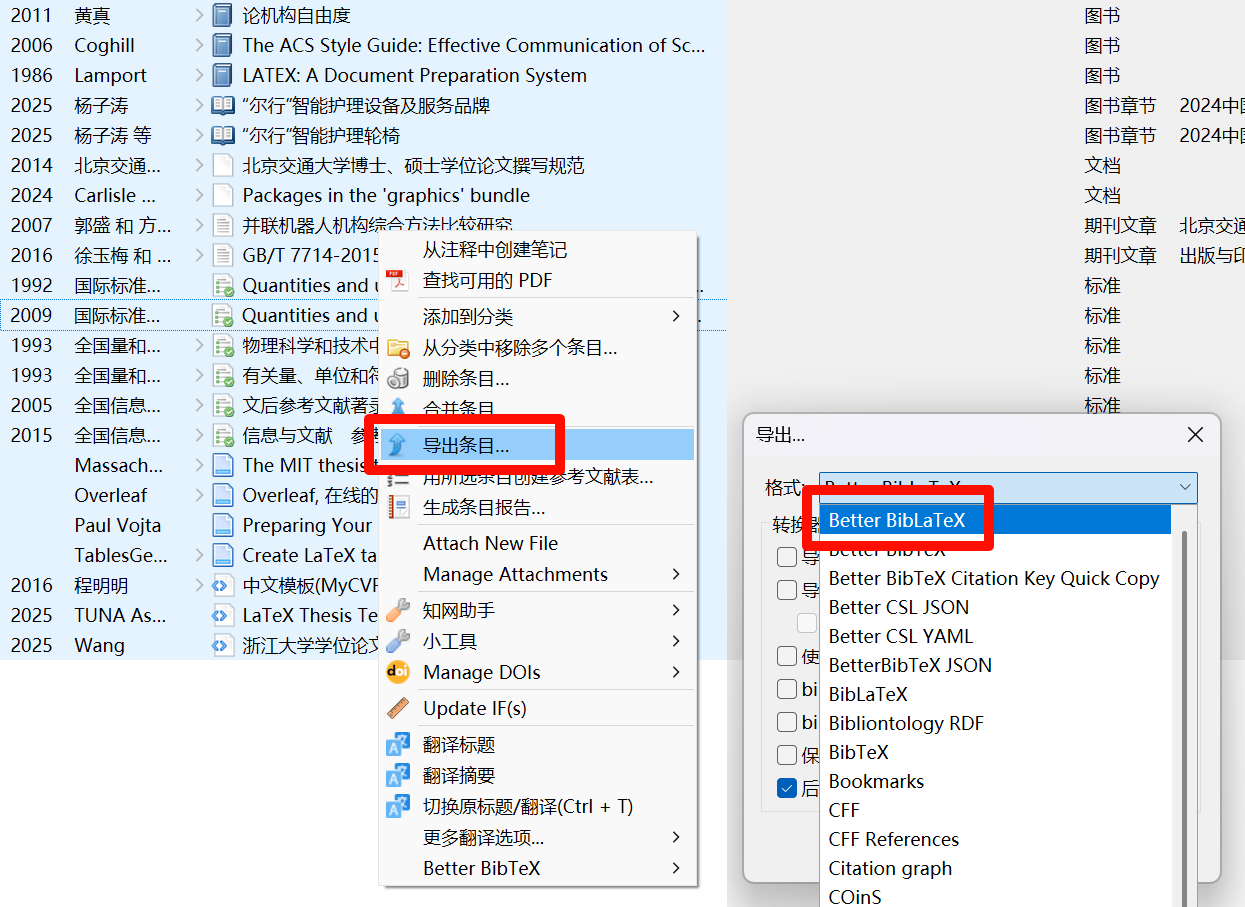
\includegraphics[width=0.8\linewidth]{figures/Zotero导出BibLaTeX流程.png}
  \bifigcaption{Zotero导出BibLaTeX流程}{The Process of Exporting BibLaTeX from Zotero}
  \label{fig:zotero}
\end{figure}

以《Sensing Expectation Enables Simultaneous Proprioception and Contact Detection in an Intelligent Soft Continuum Robot\cite{WXX+2024Sensingexpecta}》一文为例,其BibLaTeX代码为:

\begin{lstlisting}[language={BibTeX},keywordstyle={\color{Periwinkle}\bfseries}]
@article{WXX+2024Sensingexpecta,
  title = {Sensing Expectation Enables Simultaneous Proprioception and Contact Detection in an Intelligent Soft Continuum Robot},
  author = {Wang, Peiyi and Xie, Zhexin and Xin, Wenci and Tang, Zhiqiang and Yang, Xinhua and Mohanakrishnan, Muralidharan and Guo, Sheng and Laschi, Cecilia},
  date = {2024-11-18},
  journaltitle = {Nature Communications},
  shortjournal = {Nat Commun},
  volume = {15},
  number = {1},
  pages = {9978},
  publisher = {Nature Publishing Group},
  issn = {2041-1723},
  doi = {10.1038/s41467-024-54327-6},
  url = {https://www.nature.com/articles/s41467-024-54327-6},
  urldate = {2025-03-17},
}
\end{lstlisting}

在对参考文献进行引用时,在引用位置插入\cs{cite\{文献标签\}}即可。如引用上述文章的代码为:

\begin{lstlisting}[language={[LaTeX]TeX}]
    \cite{WXX+2024Sensingexpecta}
\end{lstlisting}

由于GB/T 7714-2005《文后参考文献著录规则\cite{QuanGuoXin2005WenHouCanKaoWenXianZhuLuGuiZe}》已经为过时标准,其替代标准为GB/T 7714-2015《信息与文献\quad 参考文献著录规则\cite{QuanGuoXin2015XinXiYuWenXianCanKaoWenXianZhuLuGuiZe}》,北京交通大学论文写作规范未及时更新,导致直接使用上述引用方法会有少许格式不符合学校规定。

新版本国家标准与旧版最主要的区别\cite{XuYu2016GB77142015YuGB}在于:新增了DOI号,新增了档案$[\mathrm{A}]$、舆图$[\mathrm{CM}]$、数据集$[\mathrm{DS}]$、其他$[\mathrm{Z}]$四类文献类型、用汉语拼音书写的中国著者不可缩写、标准名与标准号调换顺序、去除专利国别等。

\textbf{虽然变化如此之多,但视觉区别最大的是新增了DOI号。建议在Zotero导出前先删去“DOI号”字段(或修改gbt7714-numerical.bst文件)。同时建议对期刊、会议论文以及图书等非电子渠道独占资源删去“url”字段,虽符合旧国标与新国标,但有老师会觉得不顺眼,免得起争执。}

\subsubsection{论文内对图、表、公式、算法、章、节的引用}

在需要引用位置直接使用以下代码进行引用,不必手动输入“图”、“表”等字样:

\begin{lstlisting}[language={[LaTeX]TeX}]
    \figref{图片标签名}
    \tabref{表格标签名}
    \equref{公式标签名}
    \algref{算法标签名}
    \chptref{章标签名}
    \secref{节或子节标签名}
\end{lstlisting}

\subsubsection{脚注}

在需要脚注的位置直接使用以下代码进行脚注,每页最多10个(超过10个无法输入带圈数字\footnote{若要在其他地方输入带圈数字,可使用代码\cs{numcircled\{数字\}},该数字只能是1$\sim$10。}):

\begin{lstlisting}[language={[LaTeX]TeX}]
    \footnote{注释内容}
\end{lstlisting}


\clearpage
\section{数学符号规范}

中文论文的数学符号请务必规范处理。重点注意“标准字形”、“\textit{意大利字形}\footnote{\textit{意大利字形}(\textit{Italic Type})是拉丁字母字体排印学中的一种手写体印刷字形。因字形微向右倾斜,常被认为是西文斜体,但实际并非“斜体({\fontspec{XCharter}\hspace{-7em}\textsl{Slanting Type}})”。中文排印通常将\textit{楷体字形}与其建立对应关系。}”、“\textbf{增加字重字形}”三种字形在数学符号、上下标中的正确应用。

推荐参考GB/T 3102.11—1993《物理科学和技术中使用的数学符号\cite{QuanGuoLiang1993WuLiKeXueHeJiShuZhongShiYongDeShuXueFuHao}》、GB/T 3101—1993《有关量、单位和符号的一般原则\cite{QuanGuoLiang1993YouGuanLiangDanWeiHeFuHaoDeYiBanYuanZe}》与《The ACS Style Guide: CHAPTER 11 Numbers, Mathematics, and Units of Measure\cite{Cog2006ACSStyleGuide}》。其字形用法重点包括且不限于:

\subsection{{\kai 意大利字形(西文手写字形,对应中文楷体)}\textit{(Italic Type)}}  

\begin{enumerate}[label=(\arabic*)]
    \item \textbf{变量:} $T$代表温度,$x$代表分子分数,$r$代表速率
    \item \textbf{轴:} $y$ 轴
    \item \textbf{平面:}平面 $P$
    \item \textbf{矢量和张量的分量:} $a_x + b_x$
    \item \textbf{行列式和矩阵的元素:} $g_n$
    \item \textbf{常数:}$k_\mathrm{B}$,玻尔兹曼常数;$g$,重力加速度
    \item \textbf{描述变量的函数:}$f(x)$
    \item \textbf{定义传输属性的双字母变量:}$Kn$,Knudsen数;$Sr$,Strouhal数
\end{enumerate}


\subsection{\song 标准字形(罗马字形)(直体)(Roman Type)}

\begin{enumerate}[label=(\arabic*)]
    \item \textbf{数字}
    \item \textbf{标点符号和包围标记},如方括号、圆括号、大括号、绝对值符号等
    \item \textbf{大多数运算符},如加减乘除等号
    \item \textbf{缩写:}DoF,自由度;ARC,前交叉韧带
    \item \textbf{度量单位和时间单位:}mg,毫克;K,开尔文;Pa,帕斯卡;mmHg,毫米汞柱
    \item \textbf{非数学量或符号:} R,化学命名法中的自由基;$\mathrm{S_1}$,分子状态;s,原子轨道
    \item \textbf{变量的多字母缩写:} IP,电离电位;cmc,临界胶束浓度
    \item \textbf{数学常数:}e,自然对数的底数,2.71828...;i,虚数,$(-1)^{1/2}$;π,圆周率,3.14159...
    \item \textbf{矩阵的转置:} $\boldsymbol{A}^\mathrm{T}$($\mathrm{T}$ 是矩阵 $\boldsymbol{A}$ 的转置)
    \item \textbf{行列式:}$\mathrm{Det} \boldsymbol{A}$ 是矩阵 $\boldsymbol{A}$ 的行列式
    \item \textbf{三角函数和其他函数:}sin,lim,log,max,...
    \item \textbf{自定义运算规则:如坐标齐次变换}T()、R()、Tran()、Rot()
\end{enumerate}

\subsection{\song\textbf{增加字重字形(粗体)(Boldface Type)}}

\begin{enumerate}[label=(\arabic*)]
    \item \textbf{向量}
    \item \textbf{张量}
    \item \textbf{矩阵}
    \item \textbf{多维物理量:}$\mathbf{H}$,磁场强度
\end{enumerate}

\subsection{希腊字母(Ελληνικά Γράμματα)(Greek Letters)}
希腊字母(标准字形、\textbf{加粗字形}、\textit{意大利字形})可按字形要求用于变量、常量和向量等任何可使用拉丁字母的地方。

\subsection{Script字形(草书/书法体)与Open-Faced字形(空心/双线体)}
可以使用,但不推荐经常使用。常用的有:

\begin{enumerate}[label=(\arabic*)]
    \item \textbf{Script字形:}$\mathscr{L}$,拉格朗日量
    \item \textbf{Open-Faced字形:}$\mathbb{R}$,实数集
\end{enumerate}

\subsection{上标和下标(Subscripts and Superscripts)}

\begin{enumerate}[label=(\arabic*),itemsep=5pt]
    \item 对于本身就是物理量或数学符号的下标和上标,请使用\textit{意大利字形}。

            {\textbf{eg:\qquad }$C_p$ 表示恒压下的热容量。}

    \item 对于是缩写而不是符号的下标和上标,请使用标准字形(直体)。

            {\textbf{eg:\qquad }$C_\mathrm{B}$ 表示物体B的热容量。}
 
    \item 在大多数情况下,下标和上标最好错开。指数应放在下标之后。

            {\textbf{eg:\qquad }${C_x}^{1/2}$、$\Delta {H_1}^{\ddagger}$。\qquad 例外:$\mathrm{\lambda}_{+}^\infty$、$\mathrm{\sigma}_\mathrm{p}^+$、$B_2^{\mathrm{exptl}}$.}

    \item $\mathrm{e}^a$ 和 $\exp(a)$ 意义相同,可以互换。当以 $\mathrm{e}$ 为底数的指数很长或很复杂时,用 $\exp()$,将指数放在一行中用括弧标出。

            {\textbf{eg:\qquad }使用$\exp \left\{ \dfrac{1}{2}kT\left[ Y\left( a+b \right) -Z \right] \right\}$,避免使用$\mathrm{e}^{(1/2)kT\left[ Y\left( a+b \right) -Z \right]}.$}

    \item 在行文中,长公式避免使用根号而改用分数次幂。

            {\textbf{eg:\qquad }使用$\left[ \sinh ^2u+\left( \cosh u-1 \right) ^2 \right] ^{1/2}$,避免使用$\sqrt{ \sinh ^2u+\left( \cosh u-1 \right) ^2 }.$}
\end{enumerate}